\documentclass{article}
\usepackage[italian]{babel}
\usepackage{physics}
\usepackage{graphicx}
\usepackage{wrapfig}
\usepackage[export]{adjustbox}
\usepackage{geometry}
 \geometry{
 a4paper,
 total={170mm,257mm},
 left=20mm,
 top=20mm,
 }
\begin{document}
\title{Data Analysis for Experimental Physics with Machine Learning}

\author{A.A. 2025/26, Alessandro Foglizzo}
\date{}
\maketitle

Appunti non esaustivi del corso di Data Analysis for Experimental Physics with Machine Learning, tenuto dal prof. Paolo Meridiani presso il dipartimento di Fisica dell'Università di Torino
nell'anno 2025/2026.

\section*{Concetti fondamentali}
\begin{itemize}
    \item Dataset: insieme di coppie $(x_i,y_i)$, per i=1...N eventi
    \item Features: insieme di variabili (indice j=1...m features) che caratterizzano un evento i: $x_i=(x_{i1}, ..., x_{ij}, ..., x_{im})$
    \item Label: etichetta associata all'evento, è la variabile che lo classifice e viene utilizzata per il trainig, è il risultato atteso
    \item Modello: funzione matematica che, prendendo in pasto le features, attraverso i parametri $\theta$ ottenuti durante il training, ottiene la predizione su $\hat{y}$
    \item Funzione oggettiva: obj$(\theta)=L(\theta)+\Omega(\theta)$, misura il grado di accordo tra il fit e i dati. es MSE
    \item Loss function $L(\theta)$: misura quanto il modello è predittivo rispetto al training set $ L(\theta) = \sum_{i}(y_i-\hat{y_i})^2 $
    \item Regularization term $\Omega(\theta)$: controlla la complessità del modello e aiuta ad evitare l'overfitting
    \item variance-bias tradeoff: equilibrio tra un modello predittivo e semplice
    \item Training error: $E_{out}=Bias^2+Var+Noise$
    \item Varianza: misura quanto cambia la predizione del modello cambiando il dataset di apprendimento, e quindi la sensibilità del modello alle fluttuazioni statistiche del dataset
    \item Bias: o distorsione, indica la differenza tra le assunzioni sulla semplicità del modello e la complessità dei dati reali, ed è la differenza tra il valore predetto e quello reale
    \item Ovrefitting: alta varianza e basso bias, dato da modelli troppo complessi. Errore di training molto basso, errore di test molto alto (non generalizza)
    \item Underfitting: alto bias e bassa varianza, dato da modelli troppo semplici. Errore di training e di test molto alti.
    \item Batch: porzione/sottoinsieme del dataset di training
    \item Iperparametro: configurazione esterna al modello, che non viene appresa ma va fornita prima dell'addestramento
    \item Epoch: singola iterazione completa su tutto il dataset di addestramento
    \item Parametri di nuisance: parametri di disturbo, che rappresentano le incertezze sistematiche che possono cambiare la forma o la normalizzazione della pdf. Possono essere di natura teorica o sperimentale

\end{itemize}

\section{Neural Networks}
Estrazione automatica delle features per trovare quelle migliori per un dato task.\newline
Ogni neurone, sommando i pesi associati a ciascuna feature, misura una distanza da un iperpiano che viene non-linearizzata
per esaltarne le differenze (4.5).\newline
Diversi tipi di non linearità: Perceptron ($\theta$), sigmoide, tanh, ReLU, Leaky ReLU, ELU (4.6).\newline

L'input dei neuroni del layer denso $n$ ($z=W^Tx$) è dato dall'output (attivazioni, $a=\sigma(z)$) dei neuroni del layer $n-1$, ed ha pesi indipendenti.
Tutti i layer, meno l'input e l'output, sono nascosti (hidden): \textbf{Feed Forward Fully Connected Neural Network}.
L'output dipende dal task:
\begin{itemize}
    \item[-] Classificazione binaria: output singolo, con attivazione a sigmoide
    \item[-] Regressione lineare 1D: singolo neurone con attiivazione lineare
    \item[-] Multiclassification: K neuroni con attivazione softmax 
\end{itemize}
Senza le non linearità, i vari strati sarebbero semplificabili a una mera moltiplicazione di matrici, che dà una matrice (lineare).\newline

\textbf{Universal Approximation Theorem}: data una funzione $y=f(x)$ e un $\varepsilon>0$, esiste un deep network $y=f_w(x)$ di profondità o larghezza arbitraria per cui
\[sup||f(x)-f_w(x)||<\varepsilon\]
Quindi, una NN sufficientemente larga o profonda può approssimare una qualsiasi funzione continua su un dominio compatto. Questo però non garantisce che sia \textit{learnable}.\newline

\textbf{Training NN}:
a definita la LOSS FUNCTION in base al task e alle assunzioni: \textbf{cross-entropy} per classificazione, \textbf{MSE} per regressione.
Dopodiché, trovare i pesi $\hat{w}$ che massimizzano la massima verosimiglianza $L(w)$. Per il \textit{gradient descent}: $\pdv{L(w)}{w}$.\newline

\textbf{Backward Propagation Algorithm}: è l'algoritmo per calcolare i gradienti delle loss function. Sappiamo che che 
\[
y=f_L(...f_2(f_1(x))...)
\]
con $$y=f_L(x_L)\text{ e } x_L=f{L-1}(x_{L-1})$$
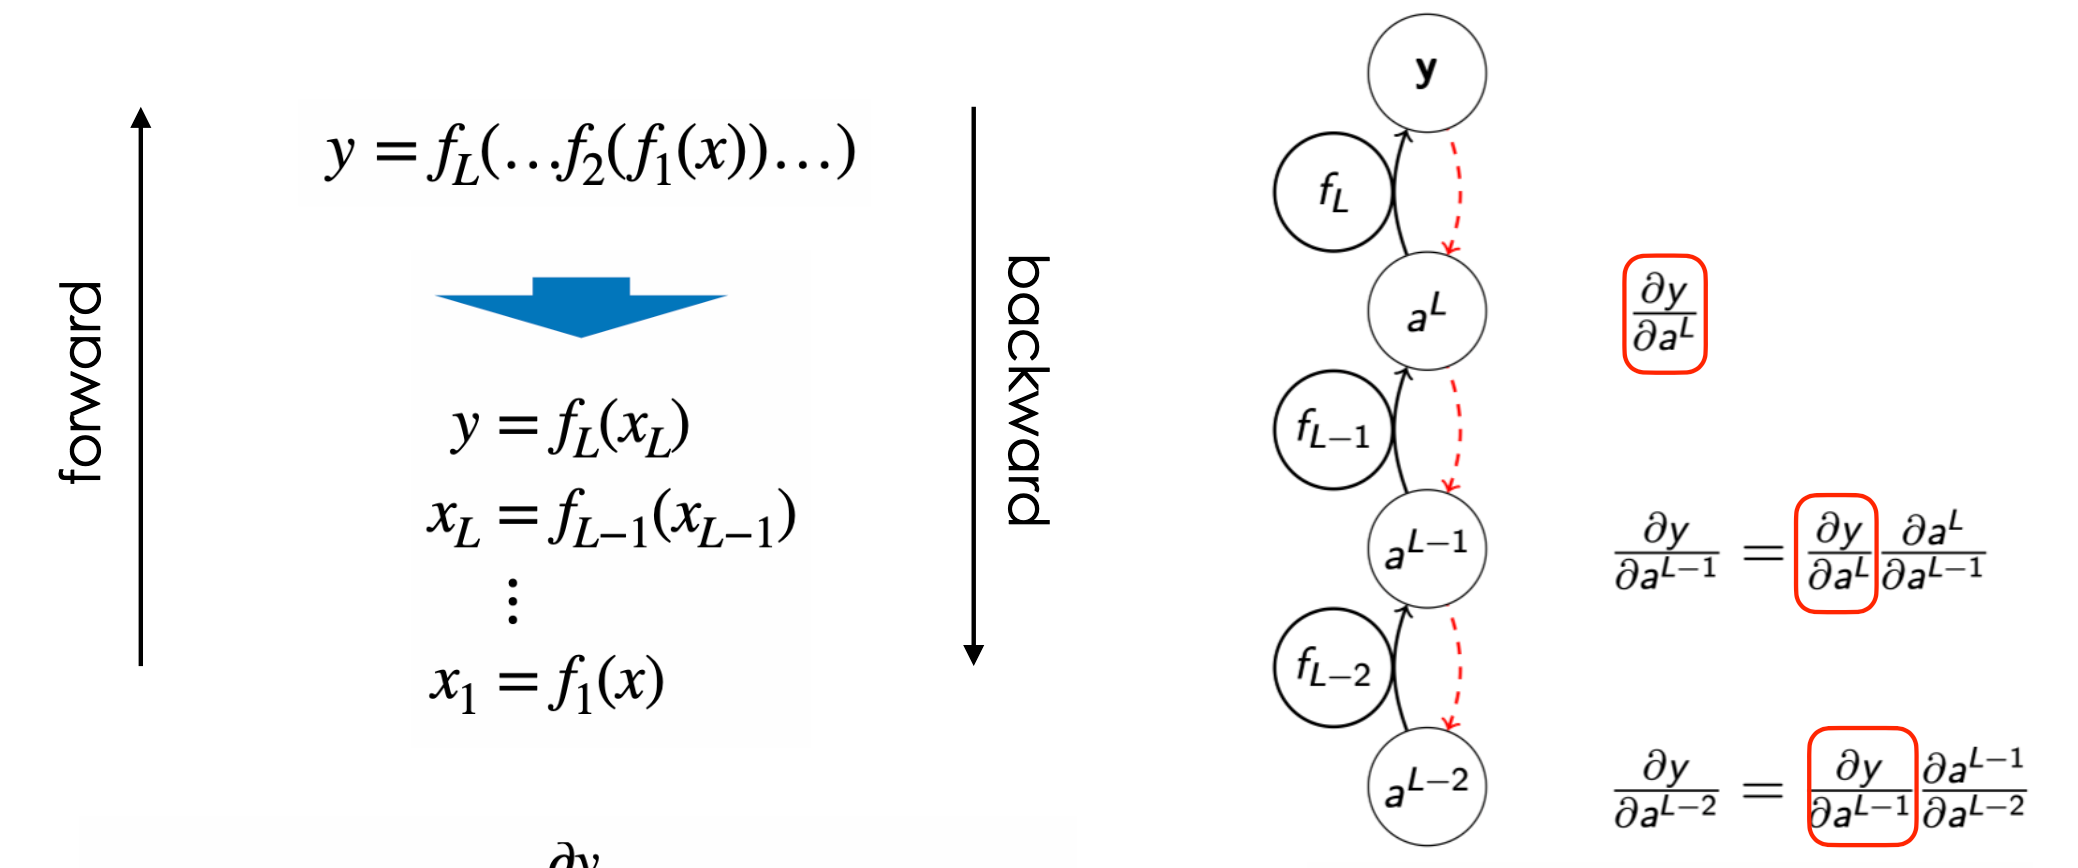
\includegraphics[width=0.7\textwidth, center]{immagini/backpropagation.png}
\newline
Per calcolare $\pdv{y}{x_l}$ con $l\in {1,...,L}$ dobbiamo applicare la chain rule.
Partendo quindi dalla derivata all'output $y=f_L$, calcoliamo a ritroso tutte le $\pdv{y}{x_l}$. (4.14)\newline
La backpropagation è fatta in automatico dalla maggior parte dei pacchetti di deep learning.
L'unica condizione per poter definire un tipo di layer è saperne definire il gradiente.\newline

Le non linearità \textit{saturating} hanno la derivata molto piccola praticamente ovunque, quindi mandano il gradiente a zero.
Inoltre la sigmoide è problematica perché non è centrata in zero e contiene un $e^x$, lento computazionalmente.\newline
Al contrario, la ReLU è molto usata e fornisce rapida convergenza e computazione; non è però centrata in zero (possibile instabilità, vedere barch normalization).

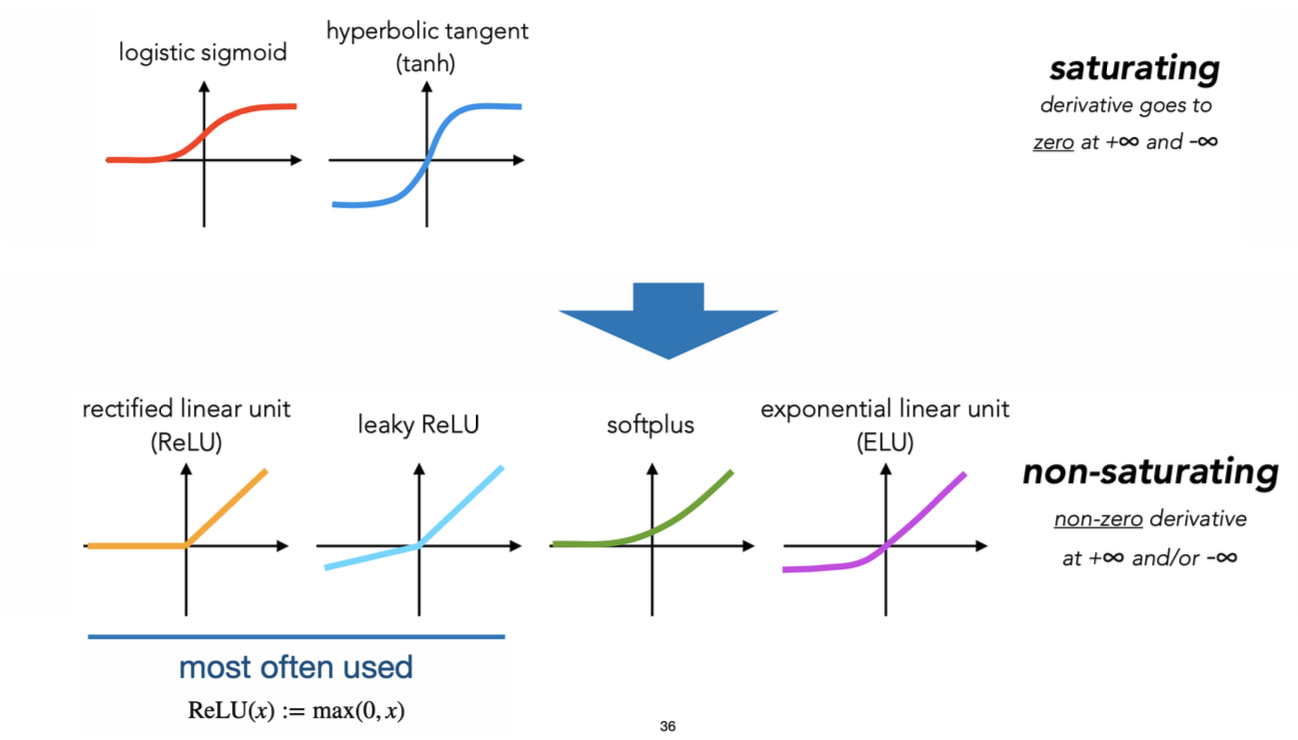
\includegraphics[width=0.7\textwidth, center]{immagini/not_and_saturating.png}

L'obiettivo dell'\textbf{inizializzazioni dei pesi} è mantenere attivazioni stabili lungo i vari layer. Vorremmo che Var($a$)$\approx$Var($z$)
per evitare che i segnali esplodano o svaniscano (vanishing gradients) durante la propagazione.\newline
Notazione:
\begin{itemize}
    \item[-] $W$: matrice dei pesi
    \item[-] $\mathcal{N}(\mu,\sigma^2)$: distribuzione normale con media $\mu$ e varianza $\sigma^2$
    \item[-] $\sim$: estratto dalla distribuzione
    \item[-] $n_{in/out}$: numero di neuroni in ingresso/uscita del layer (fan in/out)   
\end{itemize}
Esistono diverse inizializzazioni:
\begin{itemize}
    \item \textbf{Zero Initialization}: mette tutti i pesi a zero, da evitare per problemi di simmetria che impediscono l'apprendimento
    \item \textbf{Lecun Initialization}: $W\sim\mathcal{N}(0,\frac{1}{n_{in}})$
    \item \textbf{He (Kaiming) Initialization}: progettata per ReLU e Leaky ReLU, $W\sim\mathcal{N}(0,\frac{2}{n_{in}})$ (il fattore 2 compensa l'azzeramento, in media, della metà delle attivazioni)
    \item \textbf{Xavier (Glorot) Initialization}: progettata per sigmoide e tanh, $W\sim\mathcal{N}(0,\frac{1}{n_{in}+n_{out}})$ (cerca un bilanciamento tra il passo avanti e quello indietro)
\end{itemize}

\begin{wrapfigure}{l}{0.4\textwidth}
    \centering
    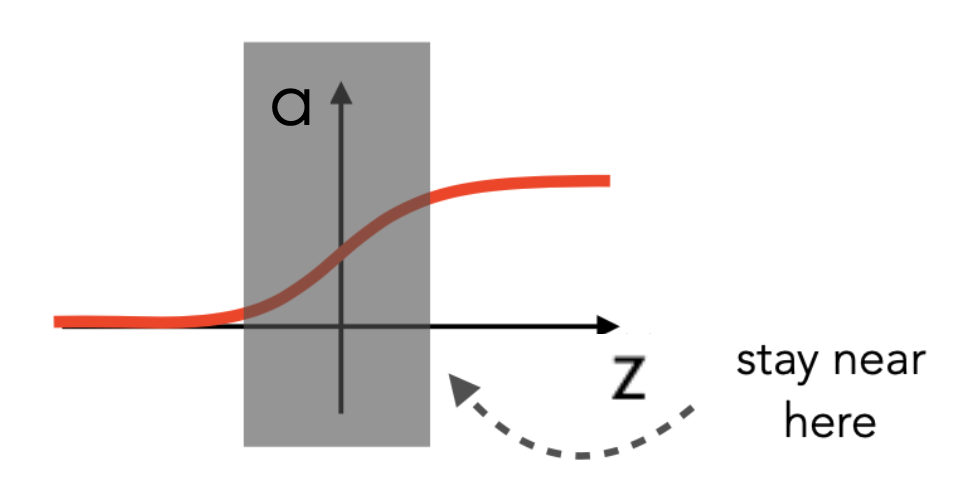
\includegraphics[width=0.35\textwidth]{immagini/batch_norm.png}
\end{wrapfigure}

\textbf{Batch Normalization}: trasformazione che riporta gli input delle attivazioni ad avere media 0 e varianza 1 e quindi rimanere all'interno del range dinamico della funzione non lineare.
Si calcola la media $\mu_B$ e la varianza $\sigma_B^2$ delle attivazioni all'interno di ogni batch, dopodiché si introducono
due parametri apprendibili: una scala $\gamma$ e uno spostamento $\beta$.

\[
\hat{x_i} = \frac{x_i-\mu_B}{\sqrt{\sigma_B^2+\varepsilon}} \qquad , \qquad y_i=\gamma \hat{x_i}+\beta
\]
La Batch Normalization sembra funzionare perché rende la loss function più smooth nei parametri.\newline
NB: utilizzando la ReLU, è comune applicare la BN \textbf{dopo} l'attivazione, perché la ReLU rimuoverebbe i valori negativi.

\textbf{Connettività Residuale}: rispetto a una rete con connettività sequenziale, in cui l'informazione deve passare attraverso tutti i layer per arrivare all'output e ogni layer trasforma completamente l'input ricevuto,
questa permette di troivare dei percorsi alternativi più brevi. Invece di imparare una funzione complessa $H(x)$, si parte da un input $x$ e si impara
solo la funzione differenza tra $H(x)$ e $x$. Matematicamente, $H(x)=F(x)+x$.
Se $x$ è già una buona approssimazione di $H(x)$, la rete dovrà solo imparare una piccola correzione $F(x)$.
\newline
In questo modo, il termine $+x$ evita che i gradienti vadano a zero e permette una backpropagation più fluida; inoltre, l'informazione è preservata anche quando $F(x)$ è molto piccola.

\textbf{Learning Rate} $\alpha$: si dovrebbe iniziare l'apprendimento con un learning rate alto, in modo da convergere più rapidamente ed evitare minimi molto pronunciati. Dopodiché, per convergere a un risultato
va diminuito il learning rate, ma non troppo presto e in più fasi in modo da evitare di finire in un minimo locale. Si possono adottare diverse strategie:
\begin{itemize}
    \item[-] Exponential Decay: decadimento graduale nel tempo, $\alpha_t=\alpha_0\exp^{-\lambda t}$
    \item[-] Cosine Annealing: riduzione graduale con una funzione coseno, $\alpha_t=\frac{1}{2}\alpha_0\left(1+\cos\left(\frac{t}{T}\pi\right)\right)$
    \item[-] 1Cycle Policy: aumenta il learning rate all'inizio, poi decade per il fine tuning  
\end{itemize}

\textbf{Riduzione dell'Overfitting (Regolarizzazione)}: tecniche di regolarizzazione per ridurre l'errore di generalizzazione limitando la complessità del modello e restringendo lo spazio dei parametri.
\begin{itemize}
    \item Early Stopping: interrompe l'addestramento se la rete non è migliorata per n epochs. Iperparametro: \textit{patience}.
    \item Dropout: impostazione di alcuni neuroni a zero, scelti randomicamente con probabilità $p$ (iperparametro). I pesi per la predizione vanno riscalati di un fattore $p$, ma è fatto in automatico dalle librerie di ML: $w_{test}(p)=p\ w_{train}(p)$
\end{itemize}

Consiglio: monitorare sempre la training history, controllando le figure di merito (loss, accuracy, MSE) per i dataset training e validazione. Inoltre, evitare numeri molto piccoli e molto grandi e controllare se ci sono NaN quando il modello non migliora.

\section{Calibrazione della risposta di un rivelatore}
Con \textbf{risposta di un rivelatore} ci si riferusce alla misura ottenuta da un rivelatore che ha ricevuto uno specifico input. I rivelatori non producono misure esatte
e per uno stesso input fisico $y$ l'output $x$ potrebbe variare per effetti stocastici (noise e risoluzione) o sistematici (soglie di misurazione,...).
Quindi, la risposta $x$ del rivelatore è governata da una legge di \textit{probabilità condizionale} $p(x|y)$.\newline

La calibrazione del detector si può formalizzare come il problema inverso, $p(y|x)$.\newline
Features in input: osservabili $x$ del rivelatore (energia ricostruita, posizione, forma degli sciami,...)\newline
Target: quantità $y$ (energia true o $\theta_{true}$, normalmente $E_{true}/E_{reco}$ o $\theta_{true}-\theta_{reco}$).\newline

Questa ricostruzione subisce tutti gli effetti del detector: noise, risoluzione, bias, non linearità. Parametrizzare $p(y|x)$ è spesso complesso, 
il goal è apprendere questa funzione per caratterizzare il comportamento del detector e correggere i bias.\newline
Una grossa sfida è data dalle distribuzioni della risposta: non gaussiane, asimmetriche e con lunghe code. Quindi la media potrebbe non corrispondere al valore più probabile.\newline

\textbf{b-jet}: gli adroni con $b$ decadono quasi sempre in adroni $c$, in parte con canali leptonici, e quindi aggiungono particelle leggere (neutrini, muoni, u/d-jets) che finiscono "fuori dal cono". Per questo, è necessaria una calibrazione specifica.
per i b-jet


\section{Classificatori per analisi di eventi HEP}
Bosone di Higgs: $m_H=125$ GeV, $\tau_H\sim10^{-25}$ s, scalare.\newline
Produzione: acccoppiamento con fermioni (in particolare t che ha la massa, e quindi l'accoppiamento con l'Higgs, maggiore) ggH (gluon fusion con loop t 90$\%$) e ttH (2g->t$\bar{\text{t}}$t$\bar{\text{t}}$); accoppiamento con bosoni vettori VBF (vector boson fusion, 2q->qqWW/qqZZ), VH (q$\bar{\text{q}}$->W/Z->W/Z+H).\newline
Decadimento nelle \textbf{Higgs Big Five}: \newline
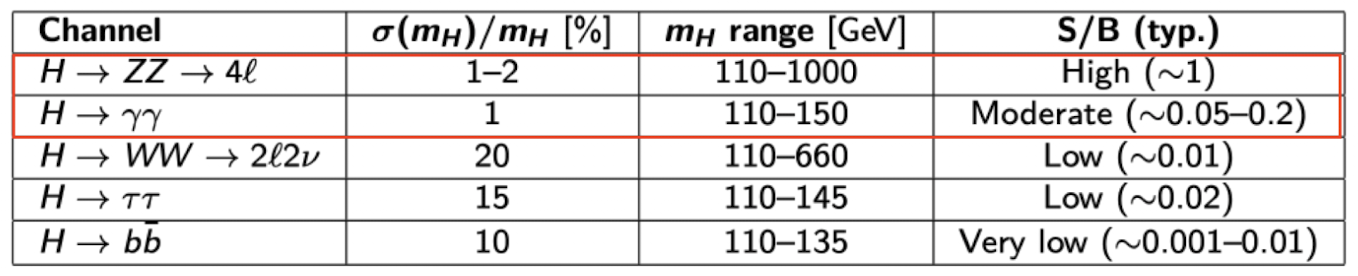
\includegraphics[width=\textwidth, center]{immagini/bigfive.png}

I canali con migliore risoluzione di massa e più grande S/B sono i più adatti per scoprire e misurare il bosone di Higgs.\newline

\textbf{Flow di un'analisi in HEP}
\begin{enumerate}
    \item Definire che cosa si vuole misurare
    \item Sceglire uno stato finale (o canale)
    \item Identificare i processi che compongono il fondo
    \item Definire come selezionare gli eventi
    \item Definire un'osservabile (numero di eventi, massa invariante, asimmetrie,...) con istogrammi
    \item Ottenere le misure e le loro incertezze
\end{enumerate}

\subsubsection*{Analisi $H\rightarrow\gamma\gamma$}
Ricerca di un picco piccolo e stretto su un grande fondo che decade esponenzialmente.
È necessaria una buona risoluzione energetica e spaziale del calorimetro EM per determinare l'angolo tra i due fotoni.\newline
\textit{Bump-Hunt Analysis}: il fondo che decade permette una stima robusta del fondo direttamente nella zona del segnale. In questo caso, su uno spettro di massa invariante $m_{\gamma\gamma}$.
\[
m_{\gamma\gamma}\sqrt{2E_1E_2(1-\cos\theta_{12})}
\]

Simple-cut analysis: selezione degli eventi che contengono 2 fotoni isolati con $p_T>30$ GeV e $\abs{\eta}<2.5$: definisce una regione di segnale usando tagi rettangolari sulle features osservabili ($p_T, \eta$, isolation).\newline
Detta $\sigma_m$ la risoluzione del picco della massa, il rapporto S/B è proporzionale a 1/$\sigma_m$: migliorare la risoluzione della massa
porta direttamente a una migliore separazione del segnale dal rumore. 
Questo si può fare con una regressione energetica (DT o NN) per correggere la risposta dell'ECAL, oppure con una stima di $\sigma_m$ evento per evento, assegnando poi i pesi maggiori agli eventi con miglior risoluzione.\newline
Un'altra via per massimizzare S/B è migliorare la selezione degli eventi, cioè riduree il False Positive Rate(FPR) mantenendo lo stesso True Positive Rate (TPR).
\begin{itemize}
    \item identificazione di fotoni isolati, per ridurre i fake-photons
    \item cinematica del sistema di-photon: usare la correlazione tra i due fotoni per separare $H\rightarrow\gamma\gamma$ dagli eventi di QCD
    \item evitare che l'output dei classificatori sia correlato alla massa invariante dei due fotoni, per mantenere il "bump-hunt"
\end{itemize}

\textbf{Di-photon classifier}: Boosted Decision Tree (BDT) addestrato su campioni simulati di segnali di Higgs (attraverso tutti i canali di produzione) e di fondo (mix di di-photons di QCD, $\gamma$+jet e di-jet fake).\newline
Per evitare che il classificatore impari ad usare la massa per discriminare i segnali, dobbiamo dare in input features che siano indipendenti da $m_{\gamma\gamma}$.\newline
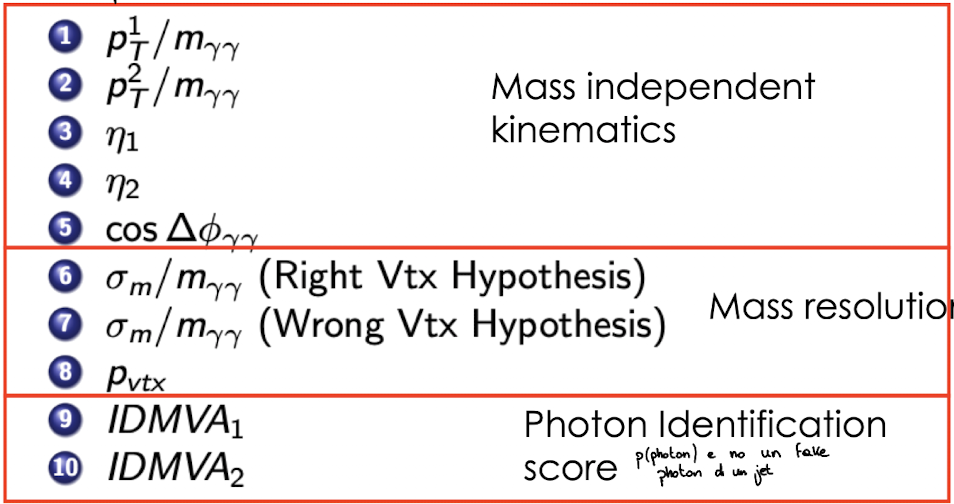
\includegraphics[width=0.6\textwidth, center]{immagini/tab_features.png}
Categorizzare gli eventi in base alla purezza del segnale migliora la sensibilità dell'intera analisi.

\textbf{Forza del segnale}: (6.16 per la funzione di likelihood con i parametri)



\end{document}